%%%%%%%%%%%%%%%%%%%%%%%%%%%%%%%%%%%%%%%%%
% The Legrand Orange Book
% LaTeX Template
% Version 2.0 (9/2/15)
% This template has been downloaded from:
% http://www.LaTeXTemplates.com
% Mathias Legrand (legrand.mathias@gmail.com) with modifications by:
% Vel (vel@latextemplates.com)
%
% License:
% CC BY-NC-SA 3.0 (http://creativecommons.org/licenses/by-nc-sa/3.0/)
%
% Important note:
% Chapter heading images should have a 2:1 width:height ratio,
% e.g. 920px width and 460px height.
%%%%%%%%%%%%%%%%%%%%%%%%%%%%%%%%%%%%%%%%%
%  Adaptado por Prof. Ausberto Castro Vera,
%  2013-2021 
%----------------------------------------------------------------------------------------
%	PACKAGES AND OTHER DOCUMENT CONFIGURATIONS
%----------------------------------------------------------------------------------------

\documentclass[11pt,fleqn]{book} % Default font size and left-justified equations

%----------------------------------------------------------------------------------------

%%%%%%%%%%%%%%%%%%%%%%%%%%%%%%%%%%%%%%%%%
% The Legrand Orange Book
% Structural Definitions File
% Version 2.0 (9/2/15)
%
% Original author:
% Mathias Legrand (legrand.mathias@gmail.com) with modifications by:
% Vel (vel@latextemplates.com)
%
% This file has been downloaded from:
% http://www.LaTeXTemplates.com
%
% License:
% CC BY-NC-SA 3.0 (http://creativecommons.org/licenses/by-nc-sa/3.0/)
%
%%%%%%%%%%%%%%%%%%%%%%%%%%%%%%%%%%%%%%%%%%

%----------------------------------------------------------------------------------------
%	VARIOUS REQUIRED PACKAGES AND CONFIGURATIONS
%----------------------------------------------------------------------------------------

\usepackage[top=3cm,bottom=3cm,left=3cm,right=3cm,headsep=10pt,a4paper]{geometry} % Page margins

\usepackage{graphicx} % Required for including pictures
\graphicspath{{Pictures/}} % Specifies the directory where pictures are stored

\usepackage{lipsum} % Inserts dummy text
\usepackage{here}   %
\usepackage{tikz} % Required for drawing custom shapes

\usepackage[brazil]{babel} % Brazilian Portuguese language/hyphenation

\usepackage{enumitem} % Customize lists
\setlist{nolistsep} % Reduce spacing between bullet points and numbered lists

\usepackage{booktabs} % Required for nicer horizontal rules in tables

\usepackage{xcolor} % Required for specifying colors by name
\definecolor{ocre}{RGB}{243,102,25} % Define the orange color used for highlighting throughout the book

\usepackage{bibentry}
%----------------------------------------------------------------------------------------
%	FONTS
%----------------------------------------------------------------------------------------

\usepackage{avant} % Use the Avantgarde font for headings
%\usepackage{times} % Use the Times font for headings
\usepackage{mathptmx} % Use the Adobe Times Roman as the default text font together with math symbols from the Sym­bol, Chancery and Com­puter Modern fonts

\usepackage{microtype} % Slightly tweak font spacing for aesthetics
\usepackage[utf8]{inputenc} % Required for including letters with accents
\usepackage[T1]{fontenc} % Use 8-bit encoding that has 256 glyphs

%----------------------------------------------------------------------------------------
%	BIBLIOGRAPHY AND INDEX
%----------------------------------------------------------------------------------------
\usepackage{hyperref}



\sloppy




%\usepackage[style=alphabetic, citestyle=numeric, sorting=nyt, sortcites=true,
%            autopunct=true, babel=hyphen, hyperref=true, abbreviate=false,
%            backref=true, backend=biber]{biblatex}
%\addbibresource{racketbib.bib} % BibTeX bibliography file
%\defbibheading{bibempty}{}

\usepackage{calc} % For simpler calculation - used for spacing the index letter headings correctly
\usepackage{makeidx} % Required to make an index
\makeindex % Tells LaTeX to create the files required for indexing

%----------------------------------------------------------------------------------------
%	MAIN TABLE OF CONTENTS
%----------------------------------------------------------------------------------------

\usepackage{titletoc} % Required for manipulating the table of contents

\contentsmargin{0cm} % Removes the default margin

% Part text styling
\titlecontents{part}[0cm]
{\addvspace{20pt}\centering\large\bfseries}
{}
{}
{}

% Chapter text styling
\titlecontents{chapter}[1.25cm] % Indentation
{\addvspace{12pt}\large\sffamily\bfseries} % Spacing and font options for chapters
{\color{ocre!60}\contentslabel[\Large\thecontentslabel]{1.25cm}\color{ocre}} % Chapter number
{\color{ocre}}
{\color{ocre!60}\normalsize\;\titlerule*[.5pc]{.}\;\thecontentspage} % Page number

% Section text styling
\titlecontents{section}[1.25cm] % Indentation
{\addvspace{3pt}\sffamily\bfseries} % Spacing and font options for sections
{\contentslabel[\thecontentslabel]{1.25cm}} % Section number
{}
{\hfill\color{black}\thecontentspage} % Page number
[]

% Subsection text styling
\titlecontents{subsection}[1.25cm] % Indentation
{\addvspace{1pt}\sffamily\small} % Spacing and font options for subsections
{\contentslabel[\thecontentslabel]{1.25cm}} % Subsection number
{}
{\ \titlerule*[.5pc]{.}\;\thecontentspage} % Page number
[]

% List of figures
\titlecontents{figure}[0em]
{\addvspace{-5pt}\sffamily}
{\thecontentslabel\hspace*{1em}}
{}
{\ \titlerule*[.5pc]{.}\;\thecontentspage}
[]

% List of tables
\titlecontents{table}[0em]
{\addvspace{-5pt}\sffamily}
{\thecontentslabel\hspace*{1em}}
{}
{\ \titlerule*[.5pc]{.}\;\thecontentspage}
[]

%----------------------------------------------------------------------------------------
%	MINI TABLE OF CONTENTS IN PART HEADS
%----------------------------------------------------------------------------------------

% Chapter text styling
\titlecontents{lchapter}[0em] % Indenting
{\addvspace{15pt}\large\sffamily\bfseries} % Spacing and font options for chapters
{\color{ocre}\contentslabel[\Large\thecontentslabel]{1.25cm}\color{ocre}} % Chapter number
{}
{\color{ocre}\normalsize\sffamily\bfseries\;\titlerule*[.5pc]{.}\;\thecontentspage} % Page number

% Section text styling
\titlecontents{lsection}[0em] % Indenting
{\sffamily\small} % Spacing and font options for sections
{\contentslabel[\thecontentslabel]{1.25cm}} % Section number
{}
{}

% Subsection text styling
\titlecontents{lsubsection}[.5em] % Indentation
{\normalfont\footnotesize\sffamily} % Font settings
{}
{}
{}

%----------------------------------------------------------------------------------------
%	PAGE HEADERS
%----------------------------------------------------------------------------------------

\usepackage{fancyhdr} % Required for header and footer configuration

\pagestyle{fancy}
\renewcommand{\chaptermark}[1]{\markboth{\sffamily\normalsize\bfseries\chaptername\ \thechapter.\ #1}{}} % Chapter text font settings
\renewcommand{\sectionmark}[1]{\markright{\sffamily\normalsize\thesection\hspace{5pt}#1}{}} % Section text font settings
\fancyhf{} \fancyhead[LE,RO]{\sffamily\normalsize\thepage} % Font setting for the page number in the header
\fancyhead[LO]{\rightmark} % Print the nearest section name on the left side of odd pages
\fancyhead[RE]{\leftmark} % Print the current chapter name on the right side of even pages
\renewcommand{\headrulewidth}{0.5pt} % Width of the rule under the header
\addtolength{\headheight}{2.5pt} % Increase the spacing around the header slightly
\renewcommand{\footrulewidth}{0pt} % Removes the rule in the footer
\fancypagestyle{plain}{\fancyhead{}\renewcommand{\headrulewidth}{0pt}} % Style for when a plain pagestyle is specified

% Removes the header from odd empty pages at the end of chapters
\makeatletter
\renewcommand{\cleardoublepage}{
\clearpage\ifodd\c@page\else
\hbox{}
\vspace*{\fill}
\thispagestyle{empty}
\newpage
\fi}

%----------------------------------------------------------------------------------------
%	THEOREM STYLES
%----------------------------------------------------------------------------------------

\usepackage{amsmath,amsfonts,amssymb,amsthm} % For math equations, theorems, symbols, etc

\newcommand{\intoo}[2]{\mathopen{]}#1\,;#2\mathclose{[}}
\newcommand{\ud}{\mathop{\mathrm{{}d}}\mathopen{}}
\newcommand{\intff}[2]{\mathopen{[}#1\,;#2\mathclose{]}}
\newtheorem{notation}{Notation}[chapter]

% Boxed/framed environments
\newtheoremstyle{ocrenumbox}% % Theorem style name
{0pt}% Space above
{0pt}% Space below
{\normalfont}% % Body font
{}% Indent amount
{\small\bf\sffamily\color{ocre}}% % Theorem head font
{\;}% Punctuation after theorem head
{0.25em}% Space after theorem head
{\small\sffamily\color{ocre}\thmname{#1}\nobreakspace\thmnumber{\@ifnotempty{#1}{}\@upn{#2}}% Theorem text (e.g. Theorem 2.1)
\thmnote{\nobreakspace\the\thm@notefont\sffamily\bfseries\color{black}---\nobreakspace#3.}} % Optional theorem note
\renewcommand{\qedsymbol}{$\blacksquare$}% Optional qed square

\newtheoremstyle{blacknumex}% Theorem style name
{5pt}% Space above
{5pt}% Space below
{\normalfont}% Body font
{} % Indent amount
{\small\bf\sffamily}% Theorem head font
{\;}% Punctuation after theorem head
{0.25em}% Space after theorem head
{\small\sffamily{\tiny\ensuremath{\blacksquare}}\nobreakspace\thmname{#1}\nobreakspace\thmnumber{\@ifnotempty{#1}{}\@upn{#2}}% Theorem text (e.g. Theorem 2.1)
\thmnote{\nobreakspace\the\thm@notefont\sffamily\bfseries---\nobreakspace#3.}}% Optional theorem note

\newtheoremstyle{blacknumbox} % Theorem style name
{0pt}% Space above
{0pt}% Space below
{\normalfont}% Body font
{}% Indent amount
{\small\bf\sffamily}% Theorem head font
{\;}% Punctuation after theorem head
{0.25em}% Space after theorem head
{\small\sffamily\thmname{#1}\nobreakspace\thmnumber{\@ifnotempty{#1}{}\@upn{#2}}% Theorem text (e.g. Theorem 2.1)
\thmnote{\nobreakspace\the\thm@notefont\sffamily\bfseries---\nobreakspace#3.}}% Optional theorem note

% Non-boxed/non-framed environments
\newtheoremstyle{ocrenum}% % Theorem style name
{5pt}% Space above
{5pt}% Space below
{\normalfont}% % Body font
{}% Indent amount
{\small\bf\sffamily\color{ocre}}% % Theorem head font
{\;}% Punctuation after theorem head
{0.25em}% Space after theorem head
{\small\sffamily\color{ocre}\thmname{#1}\nobreakspace\thmnumber{\@ifnotempty{#1}{}\@upn{#2}}% Theorem text (e.g. Theorem 2.1)
\thmnote{\nobreakspace\the\thm@notefont\sffamily\bfseries\color{black}---\nobreakspace#3.}} % Optional theorem note
\renewcommand{\qedsymbol}{$\blacksquare$}% Optional qed square
\makeatother

% Defines the theorem text style for each type of theorem to one of the three styles above
\newcounter{dummy}
\numberwithin{dummy}{section}
\theoremstyle{ocrenumbox}
\newtheorem{theoremeT}[dummy]{Theorem}
\newtheorem{problem}{Problem}[chapter]
\newtheorem{exerciseT}{Exercise}[chapter]
\theoremstyle{blacknumex}
\newtheorem{exampleT}{Example}[chapter]
\theoremstyle{blacknumbox}
\newtheorem{vocabulary}{Vocabulary}[chapter]
\newtheorem{definitionT}{Definition}[section]
\newtheorem{corollaryT}[dummy]{Corollary}
\theoremstyle{ocrenum}
\newtheorem{proposition}[dummy]{Proposition}

%----------------------------------------------------------------------------------------
%	DEFINITION OF COLORED BOXES
%----------------------------------------------------------------------------------------

\RequirePackage[framemethod=default]{mdframed} % Required for creating the theorem, definition, exercise and corollary boxes

% Theorem box
\newmdenv[skipabove=7pt,
skipbelow=7pt,
backgroundcolor=black!5,
linecolor=ocre,
innerleftmargin=5pt,
innerrightmargin=5pt,
innertopmargin=5pt,
leftmargin=0cm,
rightmargin=0cm,
innerbottommargin=5pt]{tBox}

% Exercise box	
\newmdenv[skipabove=7pt,
skipbelow=7pt,
rightline=false,
leftline=true,
topline=false,
bottomline=false,
backgroundcolor=ocre!10,
linecolor=ocre,
innerleftmargin=5pt,
innerrightmargin=5pt,
innertopmargin=5pt,
innerbottommargin=5pt,
leftmargin=0cm,
rightmargin=0cm,
linewidth=4pt]{eBox}	

% Definition box
\newmdenv[skipabove=7pt,
skipbelow=7pt,
rightline=false,
leftline=true,
topline=false,
bottomline=false,
linecolor=ocre,
innerleftmargin=5pt,
innerrightmargin=5pt,
innertopmargin=0pt,
leftmargin=0cm,
rightmargin=0cm,
linewidth=4pt,
innerbottommargin=0pt]{dBox}	

% Corollary box
\newmdenv[skipabove=7pt,
skipbelow=7pt,
rightline=false,
leftline=true,
topline=false,
bottomline=false,
linecolor=gray,
backgroundcolor=black!5,
innerleftmargin=5pt,
innerrightmargin=5pt,
innertopmargin=5pt,
leftmargin=0cm,
rightmargin=0cm,
linewidth=4pt,
innerbottommargin=5pt]{cBox}

% Creates an environment for each type of theorem and assigns it a theorem text style from the "Theorem Styles" section above and a colored box from above
\newenvironment{theorem}{\begin{tBox}\begin{theoremeT}}{\end{theoremeT}\end{tBox}}
\newenvironment{exercise}{\begin{eBox}\begin{exerciseT}}{\hfill{\color{ocre}\tiny\ensuremath{\blacksquare}}\end{exerciseT}\end{eBox}}				
\newenvironment{definition}{\begin{dBox}\begin{definitionT}}{\end{definitionT}\end{dBox}}	
\newenvironment{example}{\begin{exampleT}}{\hfill{\tiny\ensuremath{\blacksquare}}\end{exampleT}}		
\newenvironment{corollary}{\begin{cBox}\begin{corollaryT}}{\end{corollaryT}\end{cBox}}	

%----------------------------------------------------------------------------------------
%	REMARK ENVIRONMENT
%----------------------------------------------------------------------------------------

\newenvironment{remark}{\par\vspace{10pt}\small % Vertical white space above the remark and smaller font size
\begin{list}{}{
\leftmargin=35pt % Indentation on the left
\rightmargin=25pt}\item\ignorespaces % Indentation on the right
\makebox[-2.5pt]{\begin{tikzpicture}[overlay]
\node[draw=ocre!60,line width=1pt,circle,fill=ocre!25,font=\sffamily\bfseries,inner sep=2pt,outer sep=0pt] at (-15pt,0pt){\textcolor{ocre}{R}};\end{tikzpicture}} % Orange R in a circle
\advance\baselineskip -1pt}{\end{list}\vskip5pt} % Tighter line spacing and white space after remark

%----------------------------------------------------------------------------------------
%	SECTION NUMBERING IN THE MARGIN
%----------------------------------------------------------------------------------------

\makeatletter
\renewcommand{\@seccntformat}[1]{\llap{\textcolor{ocre}{\csname the#1\endcsname}\hspace{1em}}}
\renewcommand{\section}{\@startsection{section}{1}{\z@}
{-4ex \@plus -1ex \@minus -.4ex}
{1ex \@plus.2ex }
{\normalfont\large\sffamily\bfseries}}
\renewcommand{\subsection}{\@startsection {subsection}{2}{\z@}
{-3ex \@plus -0.1ex \@minus -.4ex}
{0.5ex \@plus.2ex }
{\normalfont\sffamily\bfseries}}
\renewcommand{\subsubsection}{\@startsection {subsubsection}{3}{\z@}
{-2ex \@plus -0.1ex \@minus -.2ex}
{.2ex \@plus.2ex }
{\normalfont\small\sffamily\bfseries}}
\renewcommand\paragraph{\@startsection{paragraph}{4}{\z@}
{-2ex \@plus-.2ex \@minus .2ex}
{.1ex}
{\normalfont\small\sffamily\bfseries}}

%----------------------------------------------------------------------------------------
%	PART HEADINGS
%----------------------------------------------------------------------------------------

% numbered part in the table of contents
\newcommand{\@mypartnumtocformat}[2]{%
\setlength\fboxsep{0pt}%
\noindent\colorbox{ocre!20}{\strut\parbox[c][.7cm]{\ecart}{\color{ocre!70}\Large\sffamily\bfseries\centering#1}}\hskip\esp\colorbox{ocre!40}{\strut\parbox[c][.7cm]{\linewidth-\ecart-\esp}{\Large\sffamily\centering#2}}}%
%%%%%%%%%%%%%%%%%%%%%%%%%%%%%%%%%%
% unnumbered part in the table of contents
\newcommand{\@myparttocformat}[1]{%
\setlength\fboxsep{0pt}%
\noindent\colorbox{ocre!40}{\strut\parbox[c][.7cm]{\linewidth}{\Large\sffamily\centering#1}}}%
%%%%%%%%%%%%%%%%%%%%%%%%%%%%%%%%%%
\newlength\esp
\setlength\esp{4pt}
\newlength\ecart
\setlength\ecart{1.2cm-\esp}
\newcommand{\thepartimage}{}%
\newcommand{\partimage}[1]{\renewcommand{\thepartimage}{#1}}%
\def\@part[#1]#2{%
\ifnum \c@secnumdepth >-2\relax%
\refstepcounter{part}%
\addcontentsline{toc}{part}{\texorpdfstring{\protect\@mypartnumtocformat{\thepart}{#1}}{\partname~\thepart\ ---\ #1}}
\else%
\addcontentsline{toc}{part}{\texorpdfstring{\protect\@myparttocformat{#1}}{#1}}%
\fi%
\startcontents%
\markboth{}{}%
{\thispagestyle{empty}%
\begin{tikzpicture}[remember picture,overlay]%
\node at (current page.north west){\begin{tikzpicture}[remember picture,overlay]%	
\fill[ocre!20](0cm,0cm) rectangle (\paperwidth,-\paperheight);
\node[anchor=north] at (4cm,-3.25cm){\color{ocre!40}\fontsize{220}{100}\sffamily\bfseries\@Roman\c@part};
\node[anchor=south east] at (\paperwidth-1cm,-\paperheight+1cm){\parbox[t][][t]{8.5cm}{
\printcontents{l}{0}{\setcounter{tocdepth}{1}}%
}};
\node[anchor=north east] at (\paperwidth-1.5cm,-3.25cm){\parbox[t][][t]{15cm}{\strut\raggedleft\color{white}\fontsize{30}{30}\sffamily\bfseries#2}};
\end{tikzpicture}};
\end{tikzpicture}}%
\@endpart}
\def\@spart#1{%
\startcontents%
\phantomsection
{\thispagestyle{empty}%
\begin{tikzpicture}[remember picture,overlay]%
\node at (current page.north west){\begin{tikzpicture}[remember picture,overlay]%	
\fill[ocre!20](0cm,0cm) rectangle (\paperwidth,-\paperheight);
\node[anchor=north east] at (\paperwidth-1.5cm,-3.25cm){\parbox[t][][t]{15cm}{\strut\raggedleft\color{white}\fontsize{30}{30}\sffamily\bfseries#1}};
\end{tikzpicture}};
\end{tikzpicture}}
\addcontentsline{toc}{part}{\texorpdfstring{%
\setlength\fboxsep{0pt}%
\noindent\protect\colorbox{ocre!40}{\strut\protect\parbox[c][.7cm]{\linewidth}{\Large\sffamily\protect\centering #1\quad\mbox{}}}}{#1}}%
\@endpart}
\def\@endpart{\vfil\newpage
\if@twoside
\if@openright
\null
\thispagestyle{empty}%
\newpage
\fi
\fi
\if@tempswa
\twocolumn
\fi}

%----------------------------------------------------------------------------------------
%	CHAPTER HEADINGS
%----------------------------------------------------------------------------------------

\newcommand{\thechapterimage}{}%
\newcommand{\chapterimage}[1]{\renewcommand{\thechapterimage}{#1}}%
\def\@makechapterhead#1{%
{\parindent \z@ \raggedright \normalfont
\ifnum \c@secnumdepth >\m@ne
\if@mainmatter
\begin{tikzpicture}[remember picture,overlay]
\node at (current page.north west)
{\begin{tikzpicture}[remember picture,overlay]
\node[anchor=north west,inner sep=0pt] at (0,0) {\includegraphics[width=\paperwidth]{\thechapterimage}};
\draw[anchor=west] (\Gm@lmargin,-9cm) node [line width=2pt,rounded corners=15pt,draw=ocre,fill=white,fill opacity=0.5,inner sep=15pt]{\strut\makebox[22cm]{}};
\draw[anchor=west] (\Gm@lmargin+.3cm,-9cm) node {\huge\sffamily\bfseries\color{black}\thechapter. #1\strut};
\end{tikzpicture}};
\end{tikzpicture}
\else
\begin{tikzpicture}[remember picture,overlay]
\node at (current page.north west)
{\begin{tikzpicture}[remember picture,overlay]
\node[anchor=north west,inner sep=0pt] at (0,0) {\includegraphics[width=\paperwidth]{\thechapterimage}};
\draw[anchor=west] (\Gm@lmargin,-9cm) node [line width=2pt,rounded corners=15pt,draw=ocre,fill=white,fill opacity=0.5,inner sep=15pt]{\strut\makebox[22cm]{}};
\draw[anchor=west] (\Gm@lmargin+.3cm,-9cm) node {\huge\sffamily\bfseries\color{black}#1\strut};
\end{tikzpicture}};
\end{tikzpicture}
\fi\fi\par\vspace*{270\p@}}}

%-------------------------------------------

\def\@makeschapterhead#1{%
\begin{tikzpicture}[remember picture,overlay]
\node at (current page.north west)
{\begin{tikzpicture}[remember picture,overlay]
\node[anchor=north west,inner sep=0pt] at (0,0) {\includegraphics[width=\paperwidth]{\thechapterimage}};
\draw[anchor=west] (\Gm@lmargin,-9cm) node [line width=2pt,rounded corners=15pt,draw=ocre,fill=white,fill opacity=0.5,inner sep=15pt]{\strut\makebox[22cm]{}};
\draw[anchor=west] (\Gm@lmargin+.3cm,-9cm) node {\huge\sffamily\bfseries\color{black}#1\strut};
\end{tikzpicture}};
\end{tikzpicture}
\par\vspace*{270\p@}}
\makeatother

%----------------------------------------------------------------------------------------
%	HYPERLINKS IN THE DOCUMENTS
%----------------------------------------------------------------------------------------

\usepackage{hyperref}
\hypersetup{hidelinks,backref=true,pagebackref=true,hyperindex=true,colorlinks=false,breaklinks=true,urlcolor= ocre,bookmarks=true,bookmarksopen=false,pdftitle={Title},pdfauthor={Author}}
\usepackage{bookmark}
\bookmarksetup{
open,
numbered,
addtohook={%
\ifnum\bookmarkget{level}=0 % chapter
\bookmarksetup{bold}%
\fi
\ifnum\bookmarkget{level}=-1 % part
\bookmarksetup{color=ocre,bold}%
\fi
}
}

%----------------------------------------------------------------------------------------
\usepackage[many]{tcolorbox}
\tcbset{skin=enhanced}


\usepackage{listings}
         \lstset{ %
  	      language={Scala}, % % lenguaje de programaci\'{o}n
  	      basicstyle=\bfseries\ttfamily,
  	      keywordstyle=\color{blue},
  	      commentstyle=\color{brown},	
  	      backgroundcolor=\color{green!10},
  	      showstringspaces=false
  	      }

%----------------------------------------------------------------------------------------
\usepackage[brazilian,hyperpageref]{backref}
% Configura\c{c}\~{o}es do pacote backref
% Usado sem a op\c{c}\~{a}o hyperpageref de backref
\renewcommand{\backrefpagesname}{Citado na(s) p\'{a}gina(s):~}
% Texto padr\~{a}o antes do n\'{u}mero das p\'{a}ginas
\renewcommand{\backref}{}
% Define os textos da cita\c{c}\~{a}o
\renewcommand*{\backrefalt}[4]{
	\ifcase #1 %
		Nenhuma cita\c{c}\~{a}o no texto.%
	\or
		Citado na p\'{a}gina #2.%
	\else
		Citado #1 vezes nas p\'{a}ginas #2.%
	\fi}%
% ---
%----------------------------------------------------------------------------------------
\hypersetup{
    bookmarks=true,         % show bookmarks bar?
    unicode=false,          % non-Latin characters in Acrobat’s bookmarks
    pdftoolbar=true,        % show Acrobat’s toolbar?
    pdfmenubar=true,        % show Acrobat’s menu?
    pdffitwindow=true,     % window fit to page when opened
    pdfstartview={FitH},    % fits the width of the page to the window
    pdftitle={Tutorial sobre a Linguagem Fortran},    % title
  %  pdfauthor={Mariana A. Gualhano and Ausberto S. Castro Vera},     % author
    pdfsubject={Paradigmas de Linguagens de Programa\c{c}\~{a}o},   % subject of the document
    pdfcreator={ASCV, WinEdt},   % creator of the document
    pdfproducer={ASCV}, % producer of the document
    pdfkeywords={Programa\c{c}\~{a}o} {Imperativo} {Paradigmas}, % list of keywords
    pdfnewwindow=true,      % links in new window
    colorlinks=true,       % false: boxed links; true: colored links
    linkcolor=red,          % color of internal links (change box color with linkbordercolor)
    citecolor=blue,        % color of links to bibliography
    filecolor=magenta,      % color of file links
    urlcolor=cyan           % color of external links
}	
 % Insert the commands.tex file which contains the majority of the structure behind the template

\begin{document}

%----------------------------------------------------------------------------------------
%	TITLE PAGE
%----------------------------------------------------------------------------------------

\begingroup
\thispagestyle{empty}
\begin{tikzpicture}[remember picture,overlay]
\coordinate [below=20cm] (midpoint) at (current page.north);
\node at (current page.north west)
{\begin{tikzpicture}[remember picture,overlay]
\node[anchor=north west,inner sep=0pt] at (0,0)
        {
\includegraphics[width=\paperwidth]{capa_kotlin.png}}; %Capa Imagem A4 21x29.7
\draw[anchor=north] (midpoint) node [fill=ocre!30!white,fill opacity=0.6,text opacity=1,inner sep=1cm]{\Huge\centering\bfseries\sffamily\parbox[c][][t]
        {\paperwidth}
        {\centering Introdu\c{c}\~{a}o \`{a} Linguagem Kotlin\\[5pt] % Titulo Livro
{\Large Paradigmas de Linguagens de Programa\c{c}\~{a}o}\\[20pt] % Subtitle
{\huge   \color{blue} Javier Ernesto Lopez Del Real}\\ % Autor nome
{\huge  \color{blue} Ausberto S. Castro Vera}\\
{\small \today}
}}; % Autor nome
\end{tikzpicture}};
\end{tikzpicture}
\vfill

\endgroup

%----------------------------------------------------------------------------------------
%	COPYRIGHT PAGE
%----------------------------------------------------------------------------------------

\newpage
~\vfill
\thispagestyle{empty}

\noindent Copyright \copyright\  \the\year{} Javier Ernesto  e Ausberto S. Castro Vera\\ % Copyright notice

\noindent \textsc{UENF - Universidade Estadual do Norte Fluminense Darcy Ribeiro}\\ % Universidade

\noindent \textsc{CCT - Centro de Ci\^{e}ncia e Tecnologia}\\ % Centro
\noindent \textsc{LCMAT - Laborat\'{o}rio de Matem\'{a}ticas}\\ % Laboratorio
\noindent \textsc{CC - Curso de Ci\^{e}ncia da Computa\c{c}\~{a}o}\\ % Curso

%\input{autor.tex} \\

\noindent \textit{Primeira edi\c{c}\~{a}o, Maio 2019} % Printing/edition date

%----------------------------------------------------------------------------------------
%	TABLE OF CONTENTS
%----------------------------------------------------------------------------------------

\chapterimage{sumario3.png} % Table of contents heading image

\pagestyle{empty} % No headers

\addtocontents{toc}{\protect{\pdfbookmark[0]{\contentsname}{toc}}}
\tableofcontents % Print the table of contents itself

\cleardoublepage % Forces the first chapter to start on an odd page so it's on the right

\pagestyle{fancy} % Print headers again

%----------------------------------------------------------------------------------------
%	PART
%----------------------------------------------------------------------------------------
%\part{Part One}

%----------------------------------------------------------------------------------------
%	CHAPTERS
%----------------------------------------------------------------------------------------
% Prof. Dr. Ausberto S. Castro Vera
% UENF - CCT - LCMAT - Curso de Ci\^{e}ncia da Computa\c{c}\~{a}o
% Campos, RJ,  2020
% Disciplina: Paradigmas de Linguagens de Programa\c{c}\~{a}o
% Aluno: Javier Ernesto


\chapterimage{img_superior} % Chapter heading image
\chapter{ Introdu\c{c}\~{a}o}

Kotlin é uma linguagem de programação multiplataforma,
multiparadigma, consistente e de tipagem estática, 
desenvolvido pela empresa JetBrains em 2011, que é
compilado e executado em ambiente Java na JVM 
(Java Virtual Machine). 

Ele se beneficia do aprendizado adquirido como algumas decisões de design tomadas em Java e outras línguas,
como Scala. Ele evoluiu além do que era possível com línguas mais antigas e tem
corrigido o que era doloroso sobre eles.

Atualmente a linguagem é mais 
abrangente, em fevereiro de 2012 a JetBrains  o transformou
em um projeto open source através da licença apache 2.


\section{Aspectos hist\'{o}ricos da linguagem Kotlin}
Em 2011 a linguagem de programaç\~{a}o Kotlin foi anunciada pela JetBrnais como alternativa
de escrever códigos como nas linguagens Java ou Scala que possa ser executada na Máquina Virtual do Java
(JVM). Seis anos depois o Google anunciou que Kotlin seria um caminho de 
desenvolvimento oficialmente suportado para o sistema operacional do Android.\cite{fazio2021kotlin} 

\section{\'{A}reas de Aplica\c{c}\~{a}o da Linguagem}
Ao ser compatível com a JVM (a máquina virtual do Java), 
Kotlin se torna viável como linguagem para aplicações web, 
Android, Desktop, macOS nativo e aplicativos Windows assim como Java.

Esses dois fatores são pontos de ruptura que fizeram os
desenvolvedores Android rapidamente adotar o idioma:
\begin{itemize}
	\item Kotlin é muito intuitivo e facil de aprender para desenvolvedores Java.
	A maior parter das linguagens são muito similares oa que nós ja sabemos, e as diferenças
   serão dominadas ao longo do tempo.
	
	\item Total integração com a IDE. Android Studio consegue entender,
    compilar e rodar Kotlin. Além disso, o apoio para isso
    linguagem vem da empresa que desenvolve o IDE, então nós como desenvolvedores Android
     somos cidadãos de primeira classe. 
	
\end{itemize}

Isso também quer dizer que podemos utilizar Java e Kotlin em um mesmo projeto.

Estima-se que com Kotlin a quantidade de código escrito
cai cerca de 40\% em relação ao Java. 

\subsection{ Programa\c{c}\~{a}o Cient\'{\i}fica}
A Programação Científica é uma área de estudo que,
utilizando computadores, se interessa pela
construção de modelos matemáticos e pelas técnicas 
para determinar soluções numéricas, na
análise e resolução de problemas reais
(científicos e da engenharia)

A Programação consiste, em termos práticos, na aplicação da 
simulação computacional e de outras formas de
computação, na análise e resolução de problemas 
reais em várias áreas científicas e tecnológicas.

Um exemplos de Programação Científica onde temos que implementar um 
algoritmo para calcular a norma-2 (norma Euclidiana) de um vetor x
de tamanho n, definida pela expressão (\ref*{equ1}):

\begin{center}
   \begin{equation}
      ||x||_{2} = \sqrt[]{\sum^{n}_{j=1} |x_{j}|^{2}}
      \label{equ1}
   \end{equation}
\end{center}

\chapterimage{capitulo.jpg} % Chapter heading image

% Prof. Dr. Ausberto S. Castro Vera
% UENF - CCT - LCMAT - Curso de Ci\^{e}ncia da Computa\c{c}\~{a}o
% Campos, RJ,  2020
% Disciplina: Paradigmas de Linguagens de Programa\c{c}\~{a}o
% Aluno: Javier Ernesto


\chapterimage{img_superior} % Chapter heading image ==>  Trocar este arquivo por outro 1200x468
\chapter{ Conceitos b\'{a}sicos da Linguagem Kotlin}

Em Kotlin, tudo é um objeto no sentido de que 
podemos chamar funções e propriedades de membros
 em qualquer variável. Alguns tipos podem ter uma 
 representação interna especial - por exemplo, 
 números, caracteres e booleans podem ser 
 representados como valores primitivos no tempo 
 de execução, mas para o usuário eles se parecem
 com classes comuns.
    %%%%%%%%=================================

    \section{Vari\'{a}veis e constantes}
      As variáveis em Kotlin podem ser facilmente 
    definidas como mutáveis (var) ou imutáveis (val).
    A ideia é muito semelhante ao uso "final" em variáveis Java.
    Mas a imutabilidade é um conceito muito importante em Kotlin (e muitas outras línguas modernas).
   
    Um objeto imutável é um objeto cujo estado não pode mudar 
    após a instanciação. Se você precisar de uma versão 
    modificada do objeto, um novo objeto precisa ser criado.
    Isso torna a programação muito mais robusta e previsível. 
    Em Java, a maioria dos objetos são mutáveis, o que significa
    que qualquer parte do código que tenha acesso ao objeto pode 
    modificá-lo, afetando o resto do aplicativo.

    Assim, a maneira como pensamos sobre codificação muda um pouco em Kotlin 
    se quisermos fazer uso da imutabilidade. O conceito-chave: basta usar 
    val tanto quanto possível. Haverá situações (especialmente no Android,
    onde não temos acesso ao construtor de muitas classes) onde não será 
    possível, mas será na maioria das vezes

    Outro ponto é que geralmente não precisamos 
    especificar tipos de objetos, eles serão inferidos a partir do 
    valor, o que torna o código mais limpo e mais rápido para ser modificado.
    \begin{lstlisting}
      val numero = 1 // Inteiro
      val nome = "Exemplo" // String  
    \end{lstlisting}


\section{Tipos de Dados B\'{a}sicos}
    %%%%%%%%=================================
         
 \lipsum[2]
  \subsection{Tipos Inteiros}
  Kotlin fornece um conjunto de tipos embutidos que representam números.
  Para números inteiros, existem quatro tipos com tamanhos diferentes e, portanto, faixas de valor.
    \begin{table}[ht]
      \centering
      
      \begin{tabular}{|p{2cm} p{1.5cm} p{6.0cm} p{6.0cm}| cp{2cm}}
      \hline
      \textbf{Tipo} \centering & \textbf{Size(Bits)} & \textbf{Valor mínimo} & \textbf{Valor máximo} \\ \hline
          Byte \centering    & 8  \centering  & -128   & 127                 \\ 
          Short \centering  & 16  \centering & -32768   & 32767             \\ 
          Int \centering    & 32  \centering &  -2,147,483,648 ($-2 ^{31}$)      &2,147,483,648 ($2^{31}-1$)            \\ 
          Long \centering    & 32  \centering &  -9,223,372,036,854,775,808 ($-2 ^{63}$)      &9,223,372,036,854,775,808 ($2^{63}$)              \\ \hline
      
      \end{tabular}
      \label{Tabela1}
      \end{table}
      Todas as variáveis inicializadas com valores inteiros não excedem o valor 
      máximo de ter o tipo inferido . Se o valor inicial exceder esse valor, 
      então o tipo será . Para especificar o valor explicitamente, apendice o sufixo ao valor.
     
            %%%........................

    C\'{o}digo fonte para a linguagem Kotlin:
    \begin{lstlisting}
      val one = 1 // Int
      val threeBillion = 3000000000 // Long
      val oneLong = 1L // Long
      val oneByte: Byte = 1
  
    \end{lstlisting}

    \begin{lstlisting}
  class Rational(n: Int, d: Int) {

    require(d != 0)

    private val g = gcd(n.abs, d.abs)
    val numer = n / g
    val denom = d / g

    def this(n: Int) = this(n, 1)

    def + (that: Rational): Rational =
      new Rational(
        numer * that.denom + that.numer * denom,
        denom * that.denom
      )

    def + (i: Int): Rational =
      new Rational(numer + i * denom, denom)

    def - (that: Rational): Rational =
      new Rational(
        numer * that.denom - that.numer * denom,
        denom * that.denom
      )
    \end{lstlisting}
    %%%%%%%%=================================
    \section{Operadores e Express\~{o}es em Scala}
    %%%%%%%%=================================


 

%% Prof. Dr. Ausberto S. Castro Vera
% UENF - CCT - LCMAT - Curso de Ci\^{e}ncia da Computa\c{c}\~{a}o
% Campos, RJ,  2020
% Disciplina: Paradigmas de Linguagens de Programa\c{c}\~{a}o
% Aluno: Javier Ernesto


\chapterimage{img_superior} % Chapter heading image ==>  Trocar este arquivo por outro 1200x468
\chapter{ Programa\c{c}\~{a}o em Kotlin}


%%%%%%%%======================
\section{Expressões condicionais}

\begin{lstlisting}[label={lst:example1}, language=Kotlin]
  fun maxOf(a: Int, b: Int): Int {
    if (a > b) {
        return a
    } else {
        return b
    }
}
  \end{lstlisting}
  Em Kotlin o condicional \emph{if} pode ser usado também como uma expressão:

  \begin{lstlisting}[label={lst:example1}, language=Kotlin]
    fun maxOf(a: Int, b: Int) = if (a > b) a else b
  \end{lstlisting}
  %%%%%%%%======================

%%%%%%%%======================

%%%%%%%%======================
\section{Funções}
As funções em Kotlin começam sempre com a palavra \emph{fun}. Os
parametros da função vem a variavel primeiro e em seguida vem o tipo. 
\begin{lstlisting}[label={lst:example1}, language=Kotlin]
  fun sum(a: Int, b: Int): Int {
    return a + b
}
  \end{lstlisting}

%%%%%%%%======================

\section{Classes}
Classes em Kotlin são declaradas usando-se uma palavra-chave
A declaração da classe consiste no nome da classe, no cabeçalho da
classe (especificando seus parâmetros de tipo, o construtor
primário e algumas outras coisas) e o corpo da classe entre
chaves. O cabeçalho e o corpo são opcionais; se a classe não tiver corpo, as chaves podem ser omitidas.
\begin{lstlisting}[label={lst:example1}, language=Kotlin]
      class Pessoa { /*...*/ }
      \end{lstlisting}
%%%%%%%%======================


%%%%%%%%======================
\section{Construtores}
Uma classe em Kotlin pode ter um construtor primário ou mais
 construtores secundários. O construtor primário é uma parte do
  cabeçalho da classe e vai depois do nome da classe e dos parâmetros
   de tipo opcionais.
\begin{lstlisting}[label={lst:example1}, language=Kotlin]
  class Pessoa constructor(firstName: String) { /*...*/ }
      \end{lstlisting}

Se o construtor primário não tiver anotações ou modificadores 
de visibilidade, a constructorpalavra - chave pode ser omitida:
\begin{lstlisting}[label={lst:example1}, language=Kotlin]
  class Pessoa(firstName: String) { /*...*/ }
      \end{lstlisting}
%%%%%%%%======================


%%%%%%%%======================
\section{Construtores Secundarios}
Uma classe em Kotlin pode ter um construtor primário ou mais
 construtores secundários. O construtor primário é uma parte do
  cabeçalho da classe e vai depois do nome da classe e dos parâmetros
   de tipo opcionais.
\begin{lstlisting}[label={lst:example1}, language=Kotlin]
  class Pessoa constructor(firstName: String) { /*...*/ }
      \end{lstlisting}

Se o construtor primário não tiver anotações ou modificadores 
de visibilidade, a constructorpalavra - chave pode ser omitida:
\begin{lstlisting}[label={lst:example1}, language=Kotlin]
  class Pessoa(firstName: String) { /*...*/ }
      \end{lstlisting}
%%%%%%%%======================

\subsection{Entrada e Sa\'{\i}da formatada}


%%%%%%%%======================
\section{Sele\c{c}\~{a}o}
%%%%%%%%======================
Tipos de IF

Select

%%%%%%%%======================
\section{Repeti\c{c}\~{a}o}
%%%%%%%%======================

%%%%%%%%======================
\section{Fun\c{c}\~{o}es}
%%%%%%%%======================



%%%%%%%%======================
\section{M\'{o}dulos e Subprogramas}
%%%%%%%%======================


\begin{lstlisting}
class Rational(n: Int, d: Int) {

    require(d != 0)

    val numer: Int = n
    val denom: Int = d

    def this(n: Int) = this(n, 1) // auxiliary constructor

    override def toString = numer +"/"+ denom

    def add(that: Rational): Rational =
      new Rational(
        numer * that.denom + that.numer * denom,
        denom * that.denom
      )
  }
    \end{lstlisting}


 REMOVER COMENTARIO
%% Prof. Dr. Ausberto S. Castro Vera
% UENF - CCT - LCMAT - Curso de Ci\^{e}ncia da Computa\c{c}\~{a}o
% Campos, RJ,  2020
% Disciplina: Paradigmas de Linguagens de Programa\c{c}\~{a}o
% Aluno: Javier Ernesto


\chapterimage{img_superior}
\chapter{ Aplica\c{c}\~{o}es da Linguagem Kotlin}
A linguagem de programação Kotlin é usada por mais de 60\% dos desenvolvedores Android profissionais. Ela ajuda a aumentar a produtividade, a satisfação dos desenvolvedores e a segurança do código.

\section{Android}
O Kotlin é uma linguagem compatível com Android concisa,
expressiva e projetada para ser type- e null-safe (ter segurança de tipos e de nulos). Ele funciona perfeitamente com a linguagem Java, portanto, os desenvolvedores que gostam de Java podem continuar a utilizá-lo, ao mesmo tempo que adicionam código Kotlin e usam as bibliotecas dessa linguagem. Além disso, muitos desenvolvedores Android já descobriram que o Kotlin torna o desenvolvimento mais rápido e divertido, então queremos oferecer um suporte melhor a esses usuários do Kotlin

\subsection{Hello word}
Segue um exemplo de um codigo em Kotlin no Android
mostrando o hello word.
\begin{lstlisting}[label={lst:example1}, language=Kotlin]
  public class MainActivity extends AppCompatActivity {
 
    @Override
    protected void onCreate(Bundle savedInstanceState) {
        super.onCreate(savedInstanceState);
        setContentView(R.layout.activity_main);
        TextView textView = findViewById(R.id.textView);
        Button button = findViewById(R.id.button);
        button.setOnClickListener(new View.OnClickListener() {
            @Override
            public void onClick(View v) {
                textView.setText("Hello World with Kotlin is better");
            }
        });
    }
}
}   
\end{lstlisting}


O resultado no dispositivo moile será assim:

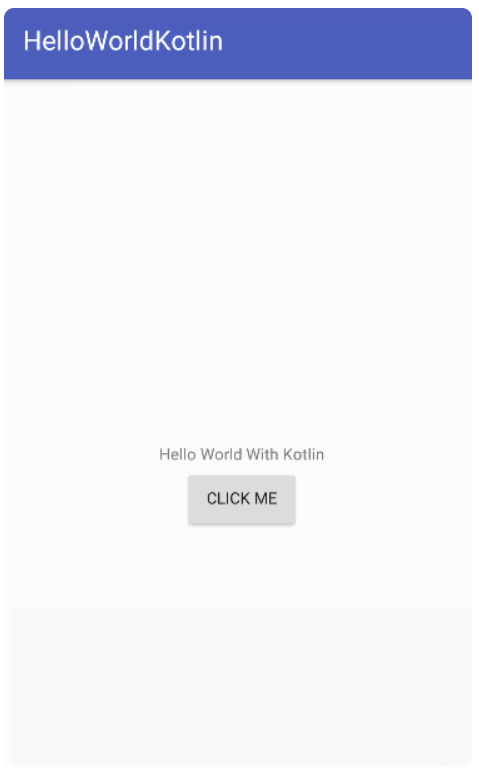
\includegraphics[ width=6cm, height=10cm]{HelloWordKotlin.PNG}


%%%--------------------------------------------------------------------
\section{O algoritmo Quicksort}
\begin{lstlisting}[label={lst:example1}, language=Kotlin]
      fun quicksort(items:List<Int>):List<Int>{
        if (items.count() < 2){
            return items
        }
        val pivot = items[items.count()/2]
        //pivot vai receber o valor central do vetor
        val equal = items.filter { it == pivot }
        //pegando o valor igual a do pivot
    
        val less = items.filter { it < pivot }
        //pegando o valor inferior ao pivot
    
        val greater = items.filter { it > pivot }
        //pegando o valor superior ao pivot

        return quicksort(less) + equal + quicksort(greater)
        //contatena os vetores e chama a funcao denovo
        }
    fun main(args: Array<String>) {
       println("Lista Original:")
        val numbers = listOf<Int>(2, 4, 7, 3, 6, 9, 5, 1, 0)
        println(numbers) //[2, 4, 7, 3, 6, 9, 5, 1, 0]
        println("Lista ordenada:")
        val ordered =  quicksort(numbers)
        println(ordered) //[0, 1, 2, 3, 4, 5, 6, 7, 9]
    }
    }   \end{lstlisting}
%%%--------------------------------------------------------------------

 REMOVER COMENTARIO
%% Prof. Dr. Ausberto S. Castro Vera
% UENF - CCT - LCMAT - Curso de Ci\^{e}ncia da Computa\c{c}\~{a}o
% Campos, RJ,  2020
% Disciplina: Paradigmas de Linguagens de Programa\c{c}\~{a}o
% Aluno: Javier Ernesto



\chapterimage{img_superior} % Chapter heading image ==>  Trocar este arquivo por outro 1200x468
\chapter{Ferramentas existentes e utilizadas}

Neste cap\'{\i}tulo devem ser apresentadas pelo menos DUAS (e no m\'{a}ximo 5) ferramentas consultadas e utilizadas para realizar o trabalho, e usar nas aplica\c{c}\~{o}es. Considere em cada caso:
\begin{itemize}
  \item Nome da ferramenta (compilador-interpretador)
  \item Endere\c{c}o na Internet
  \item Vers\~{a}o atual e utilizada
  \item Descri\c{c}\~{a}o simples (m\'{a}x 2 par\'{a}grafos)
  \item Telas capturadas da ferramenta
  \item Outras informa\c{c}\~{o}es
\end{itemize}


    \section{Editores para Fortran}


    \section{Compiladores}
            \begin{itemize}
              \item Site principal : \url{https://www.scala-lang.org/}
              \item Scala 3 : \url{https://www.scala-lang.org/download/}
              \item
              \item
              \item
            \end{itemize}



    \section{Ambientes de Programa\c{c}\~{a}o IDE para Kotlin}
 REMOVER COMENTARIO

% Prof. Dr. Ausberto S. Castro Vera
% UENF - CCT - LCMAT - Curso de Ci\^{e}ncia da Computa\c{c}\~{a}o
% Campos, RJ,  2021
% Disciplina: Paradigmas de Linguagens de Programa\c{c}\~{a}o
% Aluno: Javier Ernesto


\chapterimage{img_superior} % Chapter heading image
\chapter{Conclus\~{o}es}

Os problemas enfrentados neste trabalho ...\\
O trabalho que foi desenvolvido em forma resumida ...\\
Aspectos n\~{a}o considerados que poderiam ser estudados ou \'{u}teis para ...\\
\begin{figure}[H]
    \begin{center}
        \caption{Linguagens de programa\c{c}\~{a}o modernas e um bom livro} \label{ling2}
        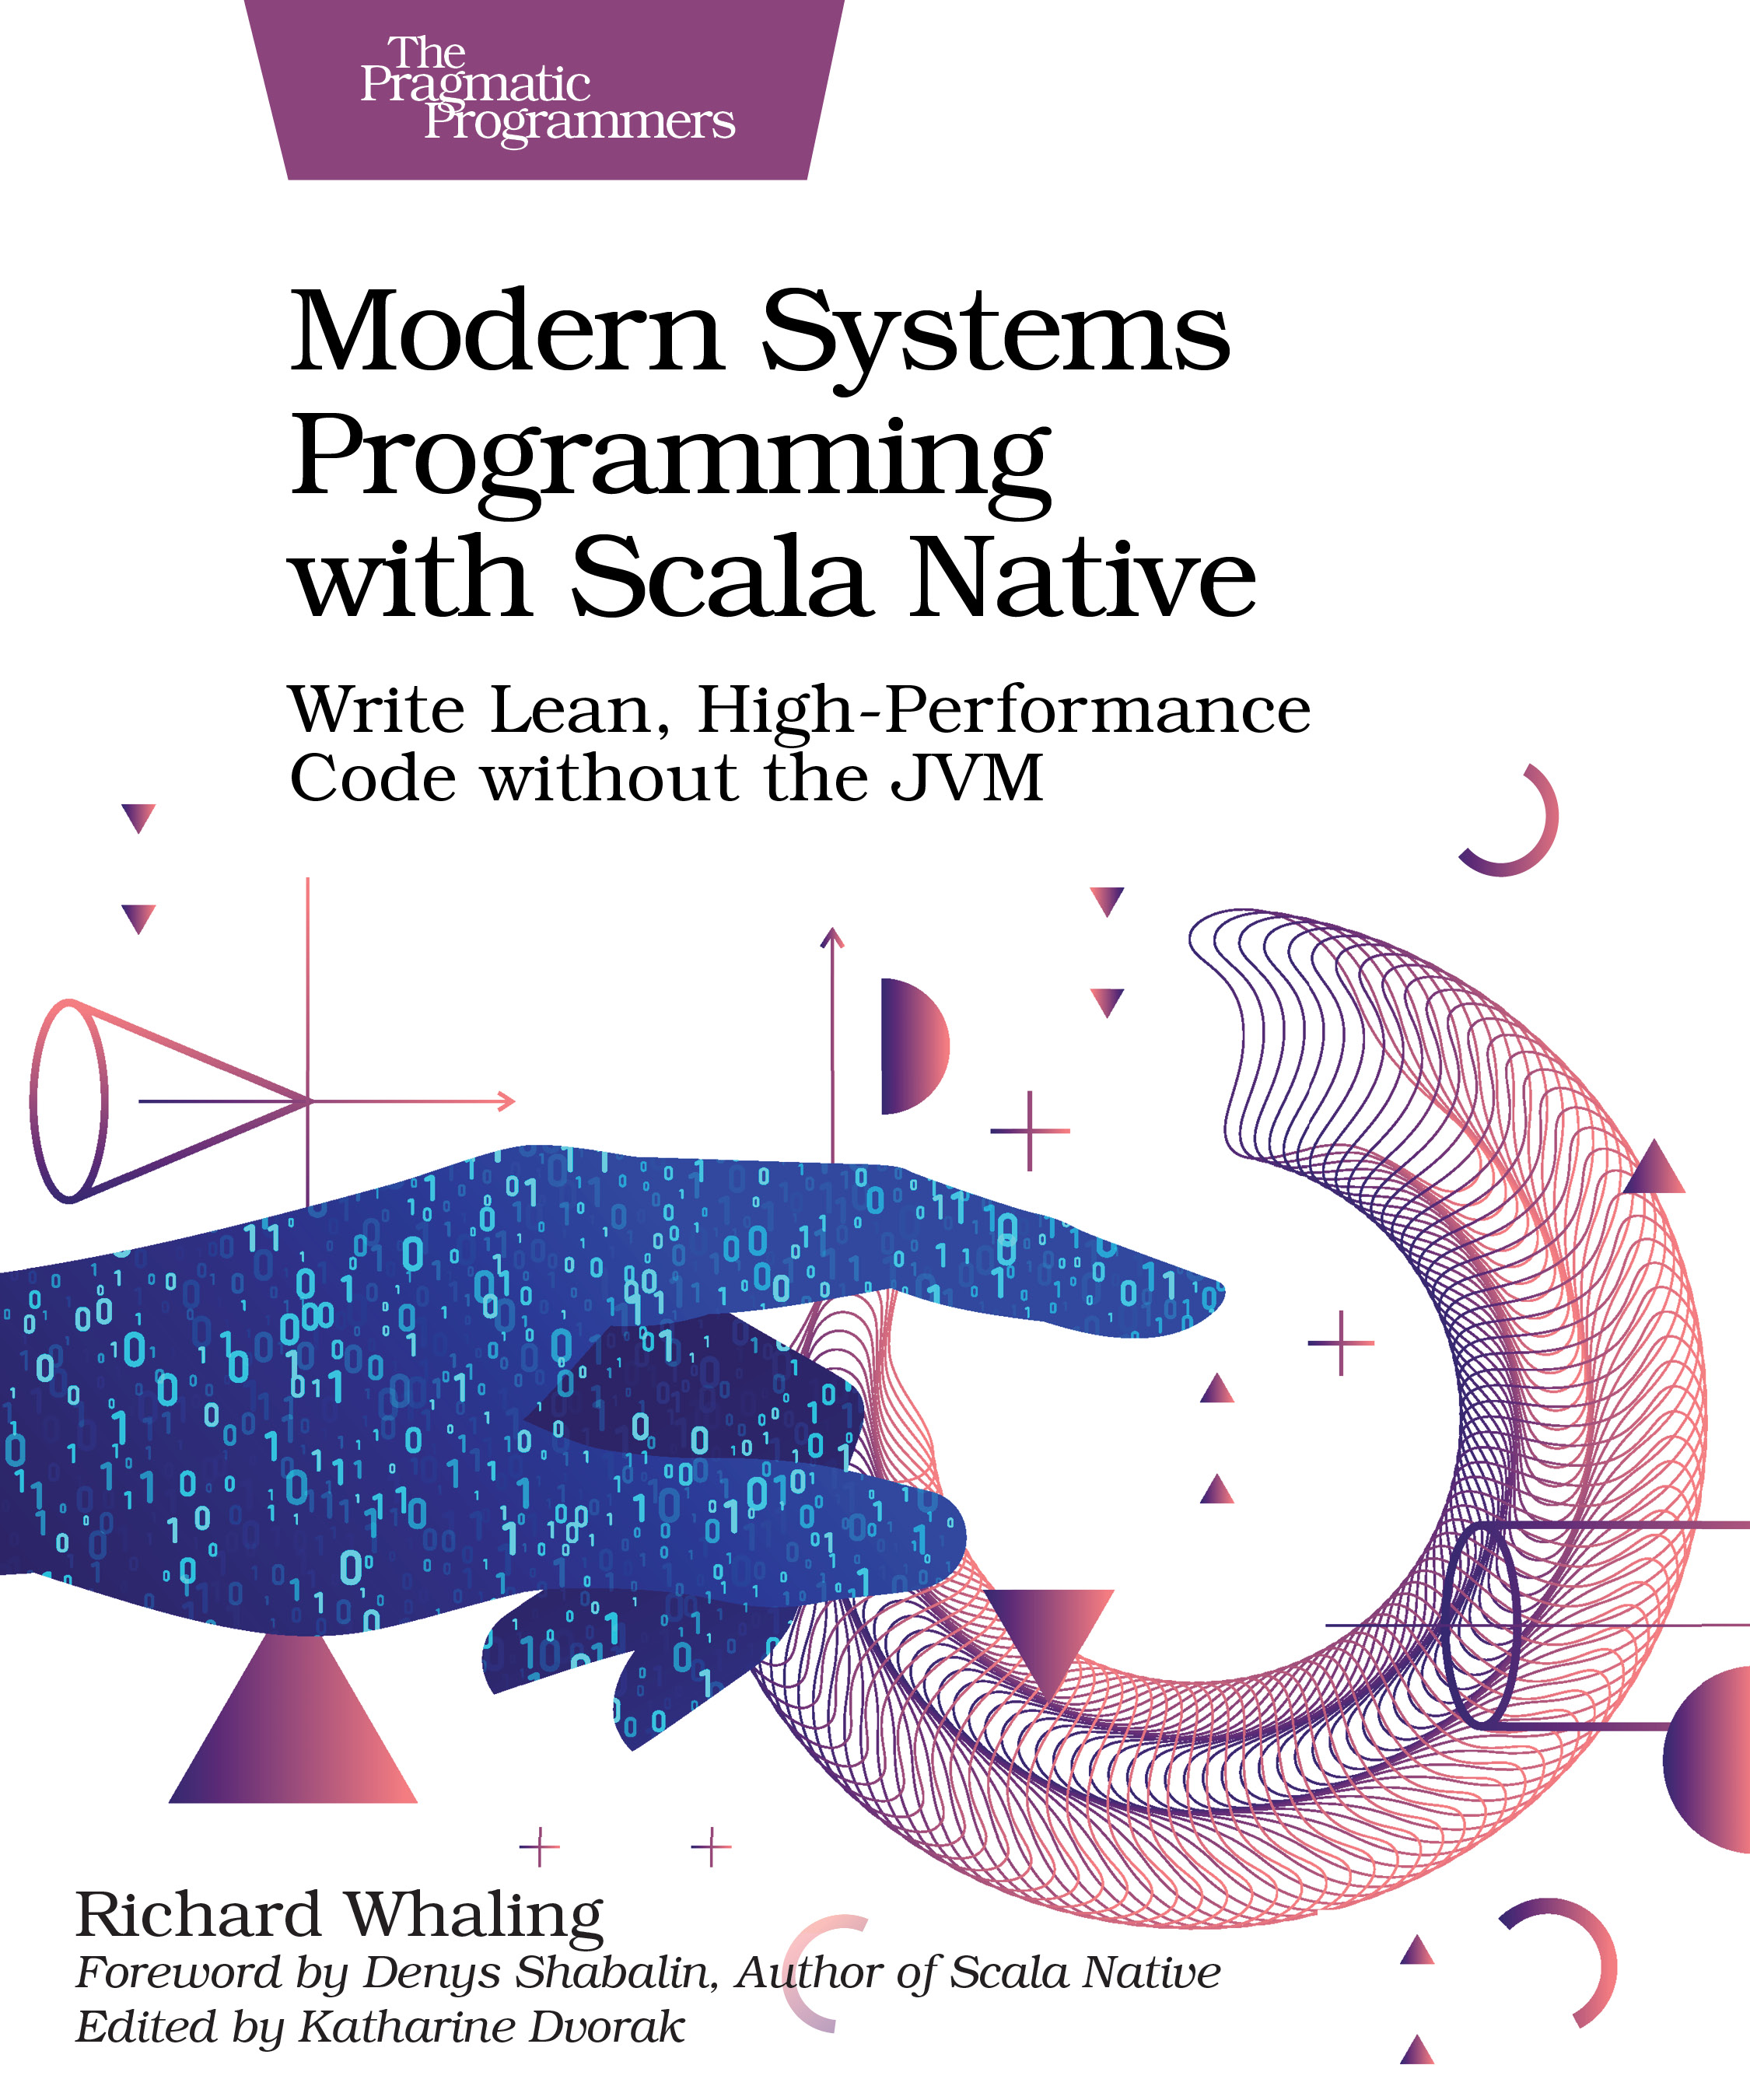
\includegraphics[width=7cm]{livro2020}
        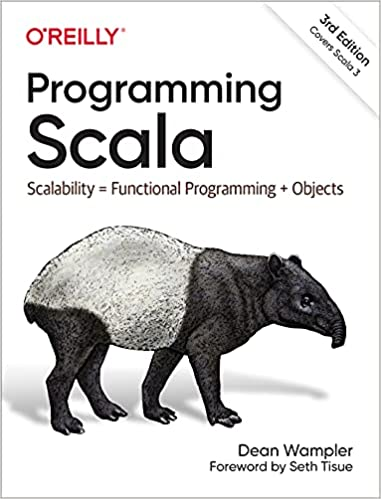
\includegraphics[width=7cm]{livro2021} \\
        {\tiny \sf Fonte: O autor }
    \end{center}
\end{figure}




\bibliographystyle{alpha}
\bibliography{Kotlin}
\addcontentsline{toc}{chapter}{\textcolor{ocre}{Bibliografia}}
%----------------------------------------------------------------------------------------
%	INDEX
%----------------------------------------------------------------------------------------

\cleardoublepage
\phantomsection
\setlength{\columnsep}{0.75cm}
\addcontentsline{toc}{chapter}{\textcolor{ocre}{Index}}
\printindex

%----------------------------------------------------------------------------------------
%% Prof. Dr. Ausberto S. Castro Vera
% UENF - CCT - LCMAT - Curso de Ci\^{e}ncia da Computa\c{c}\~{a}o
% Campos, RJ,  2021
% Disciplina: Paradigmas de Linguagens de Programa\c{c}\~{a}o
% Aluno: Javier Ernesto




\noindent
\textbf{Disciplina:} \textit{Paradigmas de Linguagens de Programa\c{c}\~{a}o \the\year}\\
\textbf{Linguagem:} \textit{Linguagem KOTLIN}\\
\textbf{Aluno:} \textit{Javier Ernesto Lopez Del Real}


\section*{Ficha de avalia\c{c}\~{a}o:}



\begin{tabular}{|p{12cm}|c|}
  \hline
  % after \\: \hline or \cline{col1-col2} \cline{col3-col4} ...
  \textbf{Aspectos de avalia\c{c}\~{a}o (requisitos m\'{\i}nimos)} & \textbf{Pontos} \\
  \hline
  Elementos b\'{a}sicos da linguagem (M\'{a}ximo: 01 pontos) &  \\
  $\bullet$ Sintaxe (vari\'{a}veis, constantes, comandos, opera\c{c}\~{o}es, etc.) &  \\
  $\bullet$ Usos e \'{a}reas de Aplica\c{c}\~{a}o da Linguagem &  \\
  \hline
  Cada elemento da linguagem (defini\c{c}\~{a}o) com exemplos (M\'{a}ximo: 02 pontos) &  \\
  $\bullet$ Exemplos com fonte diferenciada ( Courier , 10 pts, azul) & \\
  \hline
  M\'{\i}nimo 5 exemplos completos - Aplica\c{c}\~{o}es (M\'{a}ximo : 2 pontos) &  \\
  $\bullet$ Uso de rotinas-fun\c{c}\~{o}es-procedimentos, E/S formatadas &  \\
  $\bullet$ Menu de opera\c{c}\~{o}es, programas gr\'{a}ficos, matrizes, aplica\c{c}\~{o}es &  \\
  \hline
  Ferramentas (compiladores, interpretadores, etc.) (M\'{a}ximo : 2 pontos) &  \\
  $\bullet$ Ferramentas utilizadas nos exemplos: pelo menos DUAS&  \\
  $\bullet$ Descri\c{c}\~{a}o de Ferramentas existentes:  m\'{a}ximo 5&  \\
  $\bullet$ Mostrar as telas dos exemplos junto ao compilador-interpretador&  \\
  $\bullet$  Mostrar as telas dos resultados obtidos nas ferramentas &  \\
  $\bullet$ Descri\c{c}\~{a}o das ferramentas (autor, vers\~{a}o, homepage, tipo, etc.) &  \\
  \hline
  Organiza\c{c}\~{a}o do trabalho (M\'{a}ximo: 01 ponto) &  \\
  $\bullet$ Conte\'{u}do, Historia, Se\c{c}\~{o}es, gr\'{a}ficos, exemplos, conclus\~{o}es, bibliografia &  \\
  \hline
   Uso de Bibliografia (M\'{a}ximo: 01 ponto)&  \\
   $\bullet$ Livros: pelo menos 3&  \\
   $\bullet$ Artigos cient\'{\i}ficos: pelo menos 3 (IEEE Xplore, ACM Library)&  \\
   $\bullet$ Todas as Refer\^{e}ncias dentro do texto, tipo [ABC 04] & \\
   $\bullet$ Evite Refer\^{e}ncias da Internet & \\
   \hline
     &  \\
  Conceito do Professor (Opcional: 01 ponto) & \\
  \hline
   & \\
  \hfill Nota Final do trabalho: & \\
  \hline
\end{tabular}\\
\textit{Observa\c{c}\~{a}o:} Requisitos m\'{\i}nimos significa a \textit{metade} dos pontos


\end{document}

